\section{Problema aziendale}
\subsection{Descrizione generale}
L'azienda AP srl di Reggio Emilia è un'\textbf{azienda manifatturiera} specializzata nel settore metallurgico. \\
L'impresa si occupa di lavorazione, trattamento e rifinitura di metalli semilavorati in metallo e leghe per conto terzi. \\
L'azienda vuole migliorare l'efficenza dei suoi \textbf{processi produttivi} per riuscire ad essere più competitiva nel mercato.
I loro processi partono da un prodotto grezzo che deve essere lavorato da una delle macchine presenti in azienda.\\
Il processo è formato da \textbf{diverse fasi} (come si può notare anche in figura \ref{fig:fasi_di_produzione}):
\begin{enumerate}
    \item Configurazione macchina (20 min).
    \item L'operatore posiziona il prodotto grezzo in uno dei pallet dedicato della macchina. (5 min)
    \item La macchina effettua la lavorazione. (dipende dal prodotto)
    \item L'operatore controlla il prodotto lavorato, effettua i vari test qualità e sposta il prodotto finito fuori dalla macchina (10 min).
    \item Pulizia macchina (20 min).
\end{enumerate}
\begin{figure}[H]
    \centering
    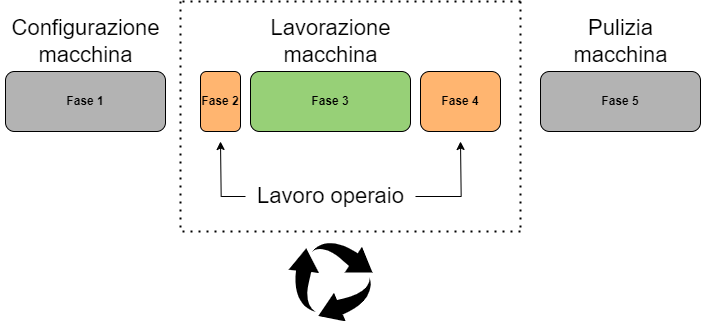
\includegraphics[width=\textwidth]{media/fasi_di_produzione.drawio.png}
    \caption{Fasi di produzione}
    \label{fig:fasi_di_produzione}
\end{figure}
Una macchina ha bisogno di essere configurata da alcuni operatori specifici, nella quale è necessario inserire il programma della lavorazione, un'attrezzatura ad hoc e i vari utensili usati dalla macchina per lavorare il prodotto.\\
Dopodiché si può iniziare la \textbf{lavorazione} vera e propria: l'operatore posiziona l'oggetto grezzo, la macchina lavora il prodotto e l'operatore controlla il lavorato facendo i vari test qualità.\\
Queste 3 fasi si \textbf{ripetono in modo ciclico} fino a quando non si raggiunge la quantità di prodotto desiderata.\\
Al termine di tutto, la macchina deve essere pulita, rimuovendo l'attrezzatura e tutti i vari utensili utilizzati, in modo da permettere una nuova configurazione.\\
Cambiare produzione di una macchina è costoso, ma è necessario farlo per poter rispettare i tempi di consegna dei clienti.\\
L'azienda vorrebbe diminuire al minimo il numero di cambi produzione sulle macchine.
\\ \\
Una macchina può avere diversi pallet e quindi gestire più lavorazioni. Non può lavorare in parallelo su più prodotti, ma è possibile parallelizzare il lavoro dell'operaio (fase 2 e 4) e quello della macchina (fase 3).\\
In questo modo si può creare una pipeline di produzione come si può notare in figura \ref{fig:pipeline_di_produzione}, dove il costo di configurazione e pulizia viene pagato una sola volta per gli n prodotti.
\begin{figure}[H]
    \centering
    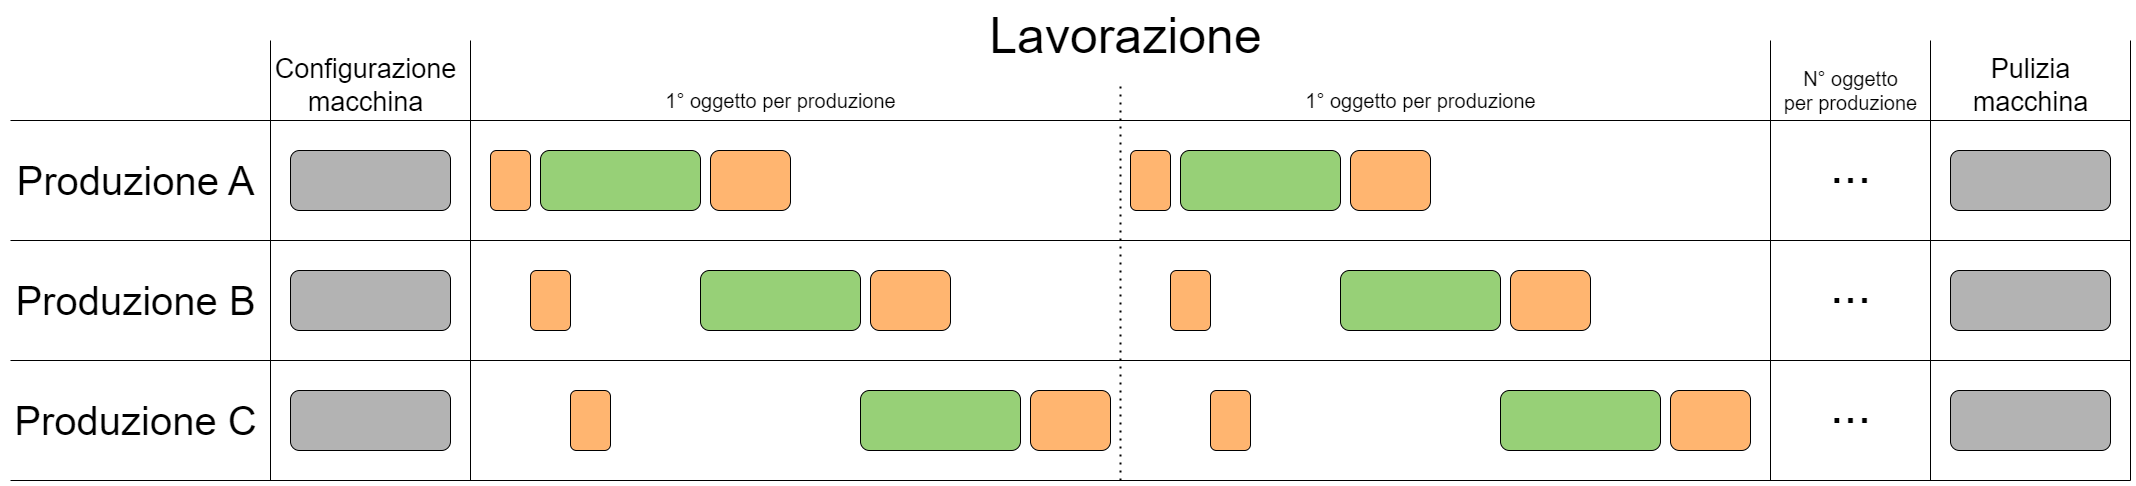
\includegraphics[width=\textwidth]{media/pipeline.drawio.png}
    \caption{Pipeline di produzione su una macchina}
    \label{fig:pipeline_di_produzione}
\end{figure}
Inoltre dopo aver posizionato il pezzo, la macchina può iniziare la lavorazione e \textbf{nel mentre} l'operatore può continuare a posizionare gli altri pezzi. 
Stesso ragionamento con il controllo qualità che può essere effettuato in parallelo con la lavorazione di un altro prodotto.\\ \\
L'azienda ha un magazzino interno per ospitare prodotti grezzi e prodotti finiti, in questo studio non viene considerata una capienza massima.\\
Nel calendario aziendale sono presenti le varie consegne dei prodotti grezzi da parte dei fornitori e le scadenze dei clienti da dover rispettare.\\

\paragraph*{Obiettivo} L'azienda vuole una \textbf{schedulazione} di N giorni (DA DECIDERE) dove per ogni giorno vengono indicate le lavorazioni da assegnare alle macchine e il numero di prodotti da ottenere. \\
La schedulazione deve rispettare i vincoli del problema e soprattuto le scadenze dei vari fornitori. \\
Inoltre deve ridurre al minimo i costi legati al cambio configurazione.

\subsection{Formalizzazione del problema}
Sono date \(n\_M\) \textbf{macchine ()} con una velocità e costo di produzione \textbf{identico} (la differenza è trascurabile), ma ognuna ha un \textbf{numero di pallet} \(n\_pallet_m\) e un \textbf{numero di utensili} \(n\_tools_m\) che può accettare (\(m \in M\)).
\\ \\
Un operaio può configurare una macchina con un certo numero di \textbf{oggetti grezzi} se il tempo di lavorazione del prodotto è maggiore di un certo \(time\_to\_parallelize\).\\
La configurazione ha sempre lo \textbf{stesso costo energetico} \(c_{conf}\): sia se si configura la macchina con 1 oggetto sia con n oggetti.
\\\\
Inoltre sono dati \(n\_W\) \textbf{tipologie di lavorazione} diverse, dove ogni lavorazione \(w \in W\) ha il \textbf{semilavorato} \(rp \in RawProducts\), il \textbf{prodotto} \(fp \in FinalProducts\), un \textbf{numero di utensili} \(n\_tools_w\) necessario e un \textbf{tempo di lavorazione macchina} \(time\_machine_w\).\\
Nella formalizzazione si definisce l'insieme generico \(P\) per riferirsi ai \textbf{prodotti} in generale presenti nel magazzino (\(P = RawProducts \cup Products\)).\\
Il \textbf{tempo} viene misurato in minuti(\(MIN\)) e giorni (\(DAYS\)).
\\\\
Nel magazzino sono presenti una quantità \(I_{tp}\) di prodotti sia grezzi che lavorati (\(t \in DAYS,\ p \in P\)). \\
L'\textbf{inventario} riceve modifiche giornaliere dalle lavorazioni decise per la giornata e riceve \textbf{incrementi} o \textbf{decrementi} dai fornitori e clienti.\\
I \textbf{fornitori} \(F_{tp}\) aggiungono una certa quantità di prodotto \(\ p \in P\) in un certo giorno \(t \in DAYS\), considerando che la mattina del giorno \(t \in DAYS\) siano già disponibili in magazzino.\\
Mentre i \textbf{clienti} \(C_{tp}\) rimuovono una certa quantità di prodotto \(\ p \in P\) in un certo giorno \(t \in DAYS\), considerando che la mattina del giorno \(t \in DAYS\) non siano più disponibili in magazzino.\\
Il magazzino non può \textbf{mai andare sotto zero} ed ha delle quantità iniziali \(I_{Op}\) e quantità finali devono essere comprese tra un minimo \(MIN\_I_{Fp}\) e un massimo \(MAX\_I_{Fp}\).

\paragraph{Differenza tra lavorazione sequenziale e lavorazione in pipeline}
La lavorazione sequenziale è quella \textbf{più costosa} sia in termini di tempo che di costo energetico.\\
Analizzando un ciclo della lavorazione in pipeline in figura \ref{fig:analisi_ciclo_di_produzione}, il tempo di lavorazione dell'operaio si paga \textbf{per un solo prodotto} rispetto agli N prodotti: fase 2 primo prodotto e fase 4 ultimo prodotto; 
mentre il restante tempo necessario alla lavorazione dell'operaio è coperto dalla lavorazione della macchina.
\begin{figure}[H]
    \centering
    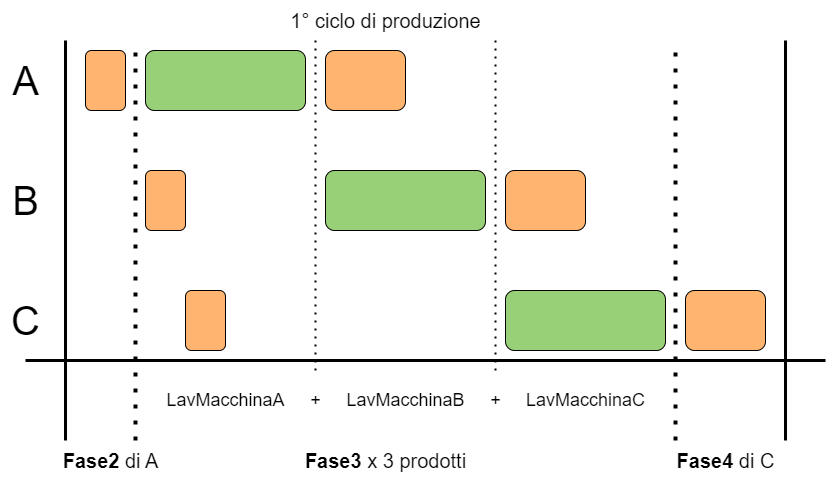
\includegraphics[width=\textwidth]{media/analisi_ciclo.drawio.png}
    \caption{Analisi singolo ciclo di produzione}
    \label{fig:analisi_ciclo_di_produzione}
\end{figure}
I tempi delle diverse fasi di produzioni possono essere semplificate come segue:
\begin{enumerate}
    \item \(time\_conf\) : tempo configurazione e pulizia macchina (fase 1 e fase 5).
    \item \(time\_operator\) : tempo di lavorazione manuale (fase 2 e fase 4).
    \item \(time\_machine_w\) : tempo di lavorazione automatica della macchina (fase 3).
\end{enumerate}
I primi due sono tempi costanti, mentre il tempo di lavorazione della macchina dipende dal prodotto da lavorare.\\
In conclusione la \textbf{differenza} tra effettuare n\_works lavorazioni sequenzialmente o in una pipeline per raggiungere N prodotti è la seguente:\\ \\
Lavorazione \textbf{sequenziale}\\ 
\begin{equation} \label{eq:TotalTimeSeq}
TotalTime = \sum_{w}^{Works} time\_conf + \left( \sum_{w}^{Works} time\_machine_w + \sum_{w}^{Works} time\_operator \right)N  
\end{equation}
\begin{equation} \label{eq:TotalCostSeq}
    TotalCost = \sum_{w}^{Works} c\_conf
\end{equation}
Lavorazione in \textbf{pipeline}\\ 
\begin{equation} \label{eq:TotalTimePipeline}
    TotalTime = time\_conf + \left( \sum_{w}^{Works} time\_machine_w + time\_operator \right) N
\end{equation}
\begin{equation} \label{eq:TotalCostPipeline}
    TotalCost = c\_conf
\end{equation}
\paragraph{Scelte dell'algoritmo}
L'algoritmo dovrà scegliere le lavorazioni da effettuare in una specifica macchina durante il giorno, ma non è importante l'ordine.\\
Queste scelte vengono definite come TASK e comprendono:
\begin{itemize}
    \item list\_works : lista delle lavorazioni.
    \item machine : macchina su cui effettuare le lavorazioni.
    \item quantity : quantità di prodotti da lavorare.
    \item day : giorno in cui fare le lavorazioni.
\end{itemize}
Per ogni attività bisogna calcolare il tempo che richiede ad essere eseguito (con le formule \ref{eq:TotalTimeSeq}  e \ref{eq:TotalTimePipeline}).\\
Se si vuole configurare un lavoro sequenziale si definiscono diversi task con un elemento in list\_works.\\
Mentre se si riesce a creare una pipeline di lavoro, allora si definisce un solo task con le varie lavorazioni in list\_works.
\\ \\
Ogni macchina può accettare diversi task giornalieri fino al raggiungimento dell'orario lavorativo massimo dell'azienda (14 ore).\\
Ad ogni definizione di una nuova attività bisogna aggiornare l'inventario del magazzino.\\
Le scelte fatte devono garantire il rispetto delle scadenze e quindi che l'inventario non vada mai sotto zero.
\\ \\
Dopo aver controllato questi vincoli, la qualità della soluzione è basata sul calcolo del costo relativo ai cambi di produzione (sommando tutte le configurazioni fatte).\\
(DA CAPIRE se aggiungere una penalità nel caso in cui si produca troppo un determinato prodotto che rimane in magazzino e\o minimizzare il tempo di lavoro).

\section{Schema del problema}
Ci sono i seguenti insiemi \textbf{Constanti}:
\begin{itemize}
    \item \(M\) : insieme di macchine
    \item \(W\) : insieme di lavorazioni
    \item \(P\) : insieme dei prodotti generico (\(RawProducts \cup Products\))
    \item \(F\) : insieme degli incrementi da parte dei fornitori
    \item \(C\) : insieme dei decrementi da parte dei clienti
\end{itemize}
Ogni \textbf{macchina} ha:
\begin{itemize}
    \item \(n\_pallet_m\) : numero pallet (numero lavorazioni in parallelo)
    \item \(n\_tools_m\) : numero utensili massimo
\end{itemize}
Ogni \textbf{lavorazione} ha:
\begin{itemize}
    \item \(n\_tools_w\) : numero utensili necessari
    \item \(time\_machine_w\) : tempo lavorazione macchina
    \item \(rp\) : prodotto grezzo
    \item \(fp\) : prodotto finale da ottenere
\end{itemize}
Ogni \textbf{prodotto} ha:
\begin{itemize}
    \item \(type\) : prodotto grezzo o finale
\end{itemize}
Ogni incremento del \textbf{fornitore} ha:
\begin{itemize}
    \item \(rp\) : prodotto grezzo
    \item \(quantity\) : quantità incrementata
    \item \(day\) : giorno di competenza
\end{itemize}
Ogni decremento del \textbf{cliente} ha:
\begin{itemize}
    \item \(fp\) : prodotto finito
    \item \(quantity\) : quantità decrementata
    \item \(day\) : giorno di competenza
\end{itemize}

\paragraph*{Configurazione dell'istanza} 
L'istanza del problema prende in considerazione:
\begin{itemize}
    \item Numero di macchine: 17 (DA DECIDERE)
    \item Numero di lavorazioni disponibili: 50 (DA DECIDERE)
    \item Giornata lavorativa: 14 ore (840 minuti)
    \item Numero giornate di schedulazioni: 30/90 (DA DECIDERE)
    \item Tempo di configurazione: 40 minuti (\(time\_conf\))
    \item Tempo lavorazione manuale\footnote{fase 2 + fase 4}: 15 minuti
    \item Tempo minimo per parallelizzare la lavorazione\footnote{\(time\_to\_parallelize\), prendendo in considerazione il tempo di lavorazione manuale con 5 minuti di tolleranza)}: 20 minuti
    \item Lista lavorazioni: DA DECIDERE.
    \item Lista macchine: DA DECIDERE.
    \item Inventario iniziale: DA DECIDERE.
    \item Inventario finale minimo e massimo: DA DECIDERE.
\end{itemize}

\paragraph{Struttura dati delle scelte}
Ci sono le seguenti \textbf{variabili}:
\begin{itemize}
    \item \(I\) : insieme dell'inventario presente in azienda
    \item \(T\) : insieme delle attività da processare nelle macchine
\end{itemize}
Ogni elemento dell'\textbf{inventario} ha:
\begin{itemize}
    \item \(day\) :  giorno di riferimento.
    \item \(p\) :  prodotto generico \(p \in P\).
    \item \(start\_quantity\) : quantità del prodotto iniziale,
    \item \(used\_quantity\) : quantità del prodotto usata (nel caso di prodotto grezzo).
    \item \(generated\_quantity\) : quantità del prodotto generata (nel caso di prodotto finito).
\end{itemize}
Con le seguenti informazioni \textbf{calcolabili}: 
\begin{equation} \label{eq:current_quantity}
    current\_quantity = start\_quantity + generated\_quantity - used\_quantity
\end{equation}
Ogni \textbf{attività} ha:
\begin{itemize}
    \item \(list\_works\) : lista delle lavorazioni.
    \item \(machine\) : macchina su cui effettuare le lavorazioni.
    \item \(quantity\) : quantità di prodotti da lavorare.
    \item \(day\) : giorno in cui fare le lavorazioni.
\end{itemize}
Con le seguenti informazioni \textbf{calcolabili}:
\begin{equation} \label{eq:genarate_quantity_fp}
    generated\_quantity_{fp} = quantity \qquad if\ fp \in list\_works, fp \in FinalProducts
\end{equation}
\begin{equation} \label{eq:used_quantity_rp}
    used\_quantity_{rp} = quantity \qquad if\ rp \in list\_works, rp \in RawProducts
\end{equation}
\begin{equation} \label{eq:time_task}
    time\_task = time\_conf + \left( \sum_{w}^{list\_works} time\_machine_w + time\_operator \right)
\end{equation}


\paragraph{Vincoli}
Tutte le variabili del problema hanno solo valori \textbf{interi e positivi}.\\
I vincoli relativi al magazzino\footnote{Nei vincoli è sottointeso \(\forall\ i \in I\) e il vincolo riguarda gli attributi di \(i\)} (\(\in I\)) sono:
\begin{itemize}
    \item Quantità iniziali uguali all'inventario iniziale definito (\ref{eq:init_start_quantity}).
    \item Quantità finali dentro il range stabilito (\ref{eq:final_current_quantity}).
    \item Tutti le quantità attuali sempre maggiori di zero (\ref{eq:current_quantity_greater_zero}).
    \item Le quantità generate sono effettivamente il risultato delle lavorazioni (\ref{eq:generate_quantity}).
    \item Le quantità usate sono effettivamente state utilizzate nella lavorazione (\ref{eq:used_quantity}).
    \item Il flusso di fornitori e clienti deve essere rispettato (\ref{eq:start_quantity}).
\end{itemize}
\begin{equation} \label{eq:init_start_quantity}
    start\_quantity_0 = I_O \qquad  \forall\ p \in P
\end{equation}
\begin{equation} \label{eq:final_current_quantity}
    MIN\_I_F <= current\_quantity_F <= MAX\_I_F \qquad  \forall\ p \in P
\end{equation}
\begin{equation} \label{eq:current_quantity_greater_zero}
    current\_quantity >= 0 \qquad \forall\ p \in P
\end{equation}
\begin{equation} \label{eq:generate_quantity}
    generated\_quantity = \sum_{q=generated\_quantity}^{t \in Task}q \qquad  \forall\ fp \in FinalProducts
\end{equation}
\begin{equation} \label{eq:used_quantity}
    used\_quantity = \sum_{q = used\_quantity}^{t \in Task}q \qquad \forall\ rp \in RawProducts
\end{equation}
\begin{equation} \label{eq:start_quantity}
    start\_quantity_{d} = current\_quantity_{d-1} + F\_quantity_{d} - C\_quantity_{d}  \qquad  \forall\ p \in P
\end{equation}
\\\\
I vincoli relativi alle attività\footnote{Nei vincoli è sottointeso \(\forall\ t \in T\) e il vincolo riguarda gli attributi di \(t\)} (\(\in T\)):
\begin{itemize}
    \item Il tempo dedicato alle macchine giornaliero deve rimanere nei limiti del'orario lavorativo giornaliero (\ref{eq:max_time_machine})
    \item Le lavorazioni (\(list\_works\)) di un'attività devono rispettare i vincoli di parallelizzazione: numero di utensili (\ref{eq:max_tools_machine}) e tempo di lavorazione adeguato (\ref{eq:min_time_to_parallelize})
\end{itemize}
\begin{equation} \label{eq:max_time_machine}
    \sum_{time\_task}^{t \in Task\_filterd(m)}time\_task \ <=\ 840 minuti \qquad  \forall\ m \in M
\end{equation}
\begin{equation} \label{eq:max_tools_machine}
    \sum_{n\_tools}^{w \in list\_machine}n\_tools_w \ <=\ n\_tools_m \qquad  m = machine \in T 
\end{equation}
\begin{equation} \label{eq:min_time_to_parallelize}
    time\_machine_w \ >=\ 20 minuti \qquad  \forall\ w \in list\_works 
\end{equation}

\paragraph{Obiettivo}
L'obiettivo è minimizzare i costi e rispettare i vincoli.
\begin{equation} \label{eq:obj}
    MIN\ \ \sum_{t}^{t \in TASK} c\_conf
\end{equation}
